\documentclass{beamer}
\beamertemplatenavigationsymbolsempty 

\title{Bad Graphs}
\subtitle{Healthcare Spending vs. Life Expectancy}

\author{Dustin Ingram}
\institute{STAT601, Summer 12-13\\ Drexel University}
\date{\today}

\begin{document}
\maketitle

\begin{frame}
    \frametitle{A bad graph, courtesy of National Geographic:}
    \begin{figure}
        \centering
        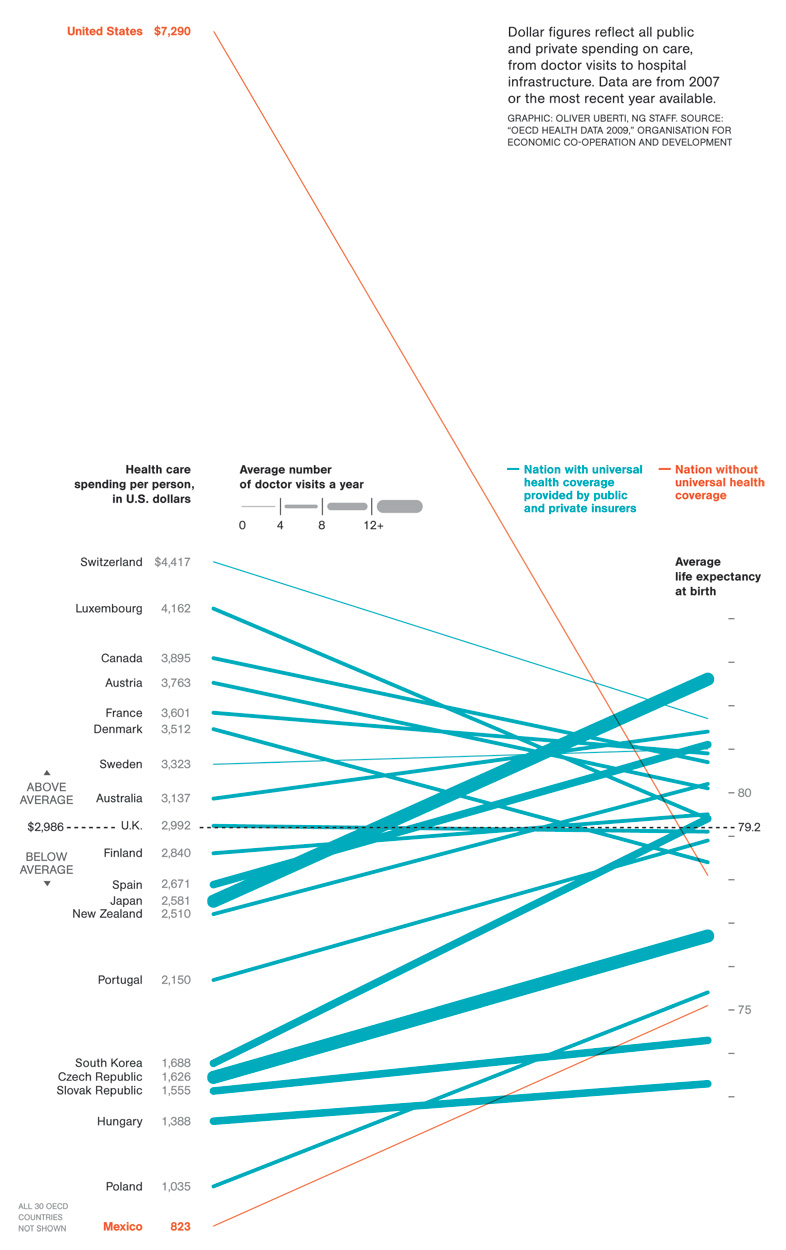
\includegraphics[height=0.8\paperheight]{original.jpg}
    \end{figure}
\end{frame}

\begin{frame}
    \frametitle{So bad, it doesn't even fit\ldots}
    \begin{figure}
        \centering
        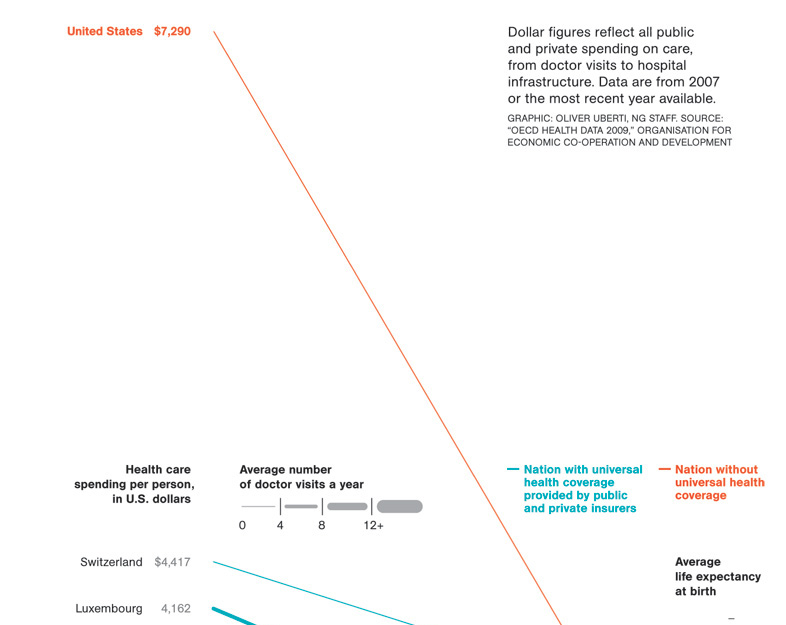
\includegraphics[width=0.8\paperwidth]{top.jpg}
    \end{figure}
\end{frame}

\begin{frame}
    \frametitle{\ldots on one slide.}
    \begin{figure}
        \centering
        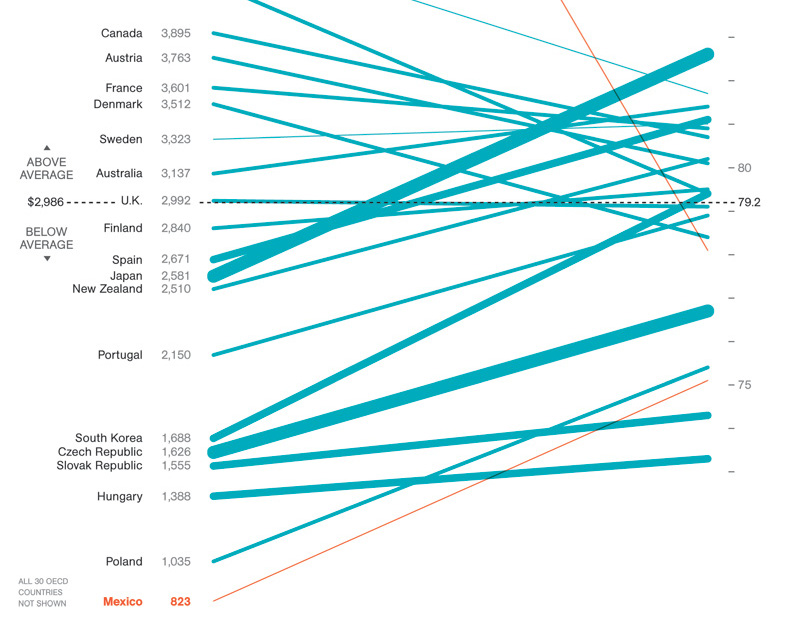
\includegraphics[width=0.8\paperwidth]{bottom.jpg}
    \end{figure}
\end{frame}

\begin{frame}
    \frametitle{Goals of this graph:}
    \begin{itemize}
        \item Show a relationship between average life expectancy and cost of healthcare for each of the OECD (Organisation for Economic Co-operation and Development) member countries;
        \item Show the average life expectancy and cost of healthcare across all of these countries;
        \item Show the average number of doctor consultations per country;
        \item Show which countries have universal healthcare, and which do not;
        \item Show that the United States is an outlier.
    \end{itemize}
\end{frame}

\begin{frame}
    \frametitle{Problems with this graph:}
    \begin{itemize}
        \item Scaling of parallel coordinate plot is arbitrary;
        \item This also makes the ``slope'' of each line arbitrary as well;
        \item Fails to show correlation between spending and life expectancy;
        \item No reason for discrete line widths, or width increments of four;
        \item Doesn't explain why some OECD countries are missing;
        \item Is it really necessary to tell the viewer which direction is ``above'' average and which is ``below''?
    \end{itemize}
\end{frame}

\begin{frame}
    \frametitle{Solution:}
    \begin{itemize}
        \item Find the original data;
        \item Use the most up-to-date, complete year (thus omitting countries with insufficient data);
        \item Use a scatter plot instead;
        \item Make the axes the average life expectancy and cost of healthcare;
        \item Make the size of the point correspond to the average number of doctor visits;
        \item Use different colors to differentiate countries with and without universal healthcare.
    \end{itemize}
\end{frame}

{
    \usebackgroundtemplate{\includegraphics[width=\paperwidth,height=\paperheight]{newgraph.pdf}}
    \begin{frame}[plain] \end{frame}
}

\begin{frame}
    \frametitle{Improvements:}
    \begin{itemize}
        \item A correlation between average life expectancy and cost of healthcare is shown;
        \item Position of individual country relative to the average life expectancy and cost of healthcare is clear;
        \item The average number of doctor consultations per country is no longer discrete;
        \item Explains why some countries are missing;
        \item The United States is very clearly an outlier.
    \end{itemize}
\end{frame}

\begin{frame}
    \frametitle{Sources:}
    \begin{itemize}
        \item Original location of the graphic:\\{\tiny\url{http://blogs.ngm.com/blog_central/2009/12/the-cost-of-care.html}}
        \item Cached version:\\{\tiny\url{http://web.archive.org/web/20130119003642/http://blogs.ngm.com/blog_central/2009/12/the-cost-of-care.html}}
        \item Cached version of the original graphic:\\{\tiny\url{http://web.archive.org/web/20130116193447/http://blogs.ngm.com/.a/6a00e0098226918833012876a6070f970c-800wi}}
        \item Source of the data:\\{\tiny\url{http://www.oecd.org/els/health-systems/oecdhealthdata2013-frequentlyrequesteddata.htm}}
    \end{itemize}
\end{frame}

\end{document}
